\documentclass{standalone}
\usepackage{tikz}
\begin{document}
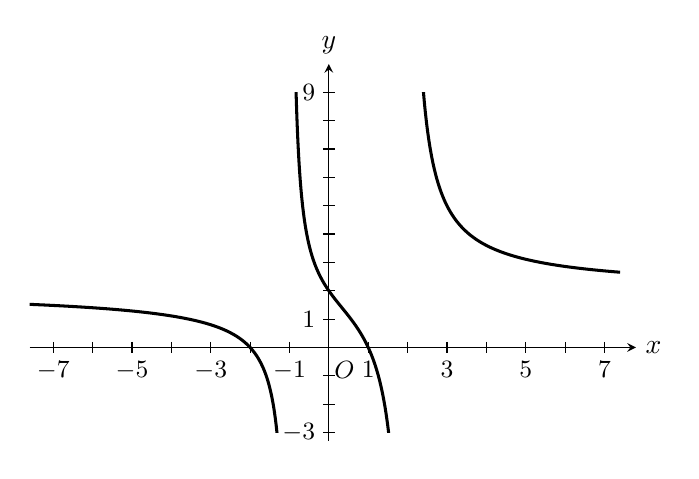
\begin{tikzpicture}[color=black, >=stealth, x=0.5cm, y=0.36cm]
  % Axes with a tick at every integer
  \draw[->] (-7.6,0) -- (7.8,0) node[right] {$x$};
  \draw[->] (0,-3.3) -- (0,10) node[above] {$y$};
  \foreach \x in {-7,...,7} \draw (\x,0.2) -- (\x,-0.2);
  \foreach \y in {-3,...,9} \draw (0.15,\y) -- (-0.15,\y);
  % Tick labels
  \foreach \x in {-7,-5,-3,-1,1,3,5,7}
    \node[font=\small, below] at (\x,-0.15) {$\x$};
  \node[font=\small, below] at (0.4,-0.15) {$O$};
  \foreach \y in {-3,1,9}
    \node[font=\small, left] at (-0.1,\y) {$\y$};
  % Three branches; zeros at x = -2 and x = 1, y-intercept 2,
  % vertical asymptotes near x = -1 and x = 2 (not drawn in original)
  \begin{scope}
    \clip (-7.6,-3) rectangle (7.6,9);
    \draw[line width=1.1pt, smooth, samples=150, domain=-7.6:-1.25]
      plot (\x, {2*(\x+2)*(\x-1)/((\x+1)*(\x-2))});
    \draw[line width=1.1pt, smooth, samples=200, domain=-0.84:1.55]
      plot (\x, {2*(\x+2)*(\x-1)/((\x+1)*(\x-2))});
    \draw[line width=1.1pt, smooth, samples=150, domain=2.38:7.4]
      plot (\x, {2*(\x+2)*(\x-1)/((\x+1)*(\x-2))});
  \end{scope}
\end{tikzpicture}
\end{document}
